Consider the matrix  $A = \begin{bmatrix} 1 & 0\\ 2  & 1 \\ 0 & 1 \end{bmatrix}$.

\begin{enumerate}
    \item Define the matrix $B = AA^{\top}$, compute the matrix $B$.

    \item Show that the following is an Eigendecomposition of the matrix $B$:
    \begin{align*}
      \begin{bmatrix} \frac{-2}{\sqrt{30}} & \frac{1}{\sqrt{5}} & \frac{2}{\sqrt{6}}\\ \frac{-5}{\sqrt{30}} & 0 & \frac{-1}{\sqrt{6}} \\ \frac{-1}{\sqrt{30}} & \frac{-2}{\sqrt{5}} & \frac{1}{\sqrt{6}} \end{bmatrix}
      \begin{bmatrix} 6 & 0 & 0\\ 0 & 1 & 0 \\ 0 & 0 & 0 \end{bmatrix}
      \begin{bmatrix} \frac{-2}{\sqrt{30}} & \frac{-5}{\sqrt{30}} & \frac{-1}{\sqrt{30}} \\ \frac{1}{\sqrt{5}} & 0 & \frac{-2}{\sqrt{5}} \\ \frac{2}{\sqrt{6}}  & \frac{-1}{\sqrt{6}} & \frac{1}{\sqrt{6}}  \end{bmatrix}
    \end{align*}

    \item Find the singular value matrix for A. That is, if $A = U \Sigma V^{\top}$ is the SVD of $A$, find $\Sigma$.

    \item Consider a SVD of a matrix $D$ as follows:
    \begin{align*}
        D = \begin{bmatrix} \frac{1}{2} & \frac{-\sqrt{3}}{2} \\ \frac{\sqrt{3}}{2} & \frac{1}{2} \end{bmatrix} \begin{bmatrix} 4 & 0 \\ 0 & 1/2 \end{bmatrix} 
        \begin{bmatrix} \frac{\sqrt{2}}{2} & \frac{\sqrt{2}}{2} \\ \frac{-\sqrt{2}}{2} & \frac{\sqrt{2}}{2} \end{bmatrix}^\top
    \end{align*}

    A matrix $R_\theta \in \mathbb{R}^{2\times 2}$ is a 2D rotation matrix if it has the following form:
    \begin{align*}
        R_\theta = \begin{bmatrix} \cos{\theta} & -\sin{\theta} \\ \sin{\theta} & \cos{\theta} \end{bmatrix}
    \end{align*}
    where $\theta \in \mathbb{R}$. Geometrically speaking, $R_{\theta} \vv{v}$ rotates $\vv{v}$ counterclockwise by angle $\theta$, for any  $\vv{v} \in \mathbb{R}^2$, as shown in Figure \ref{rotation}.
    \begin{center}
    \captionsetup[figure]{font=small}
    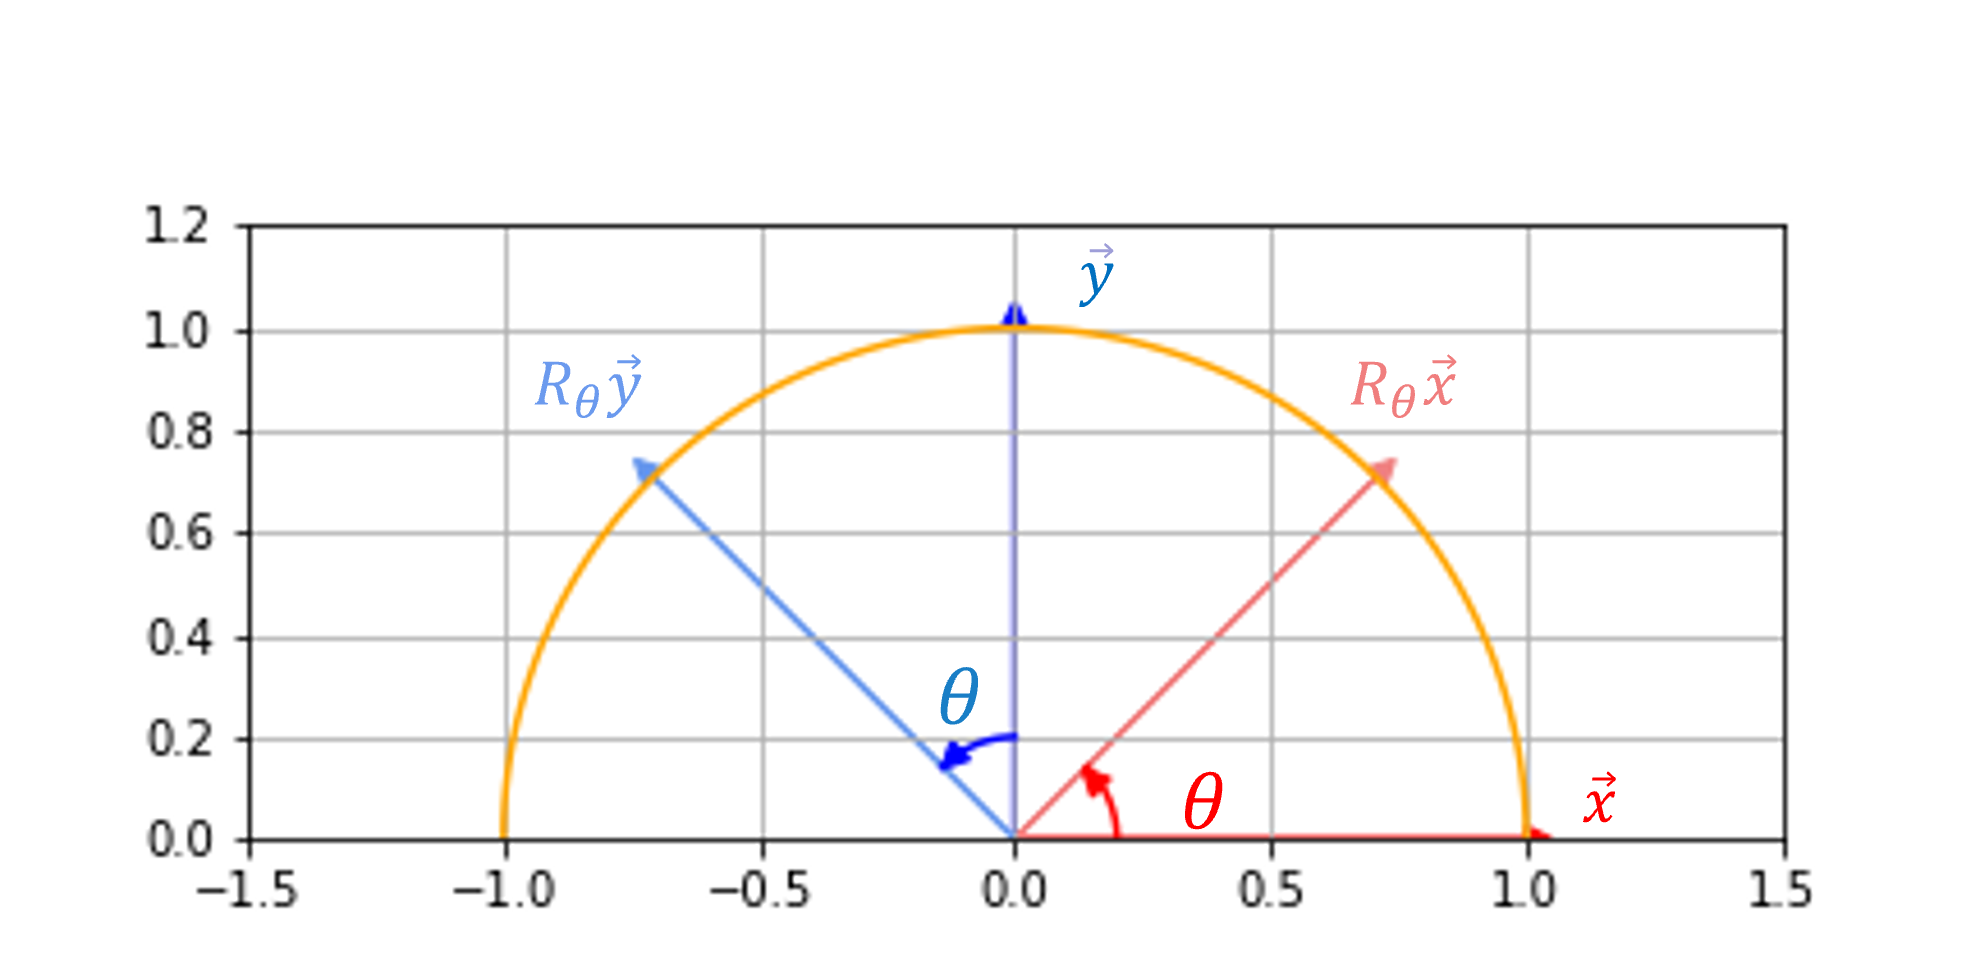
\includegraphics[scale=0.7]{figs/rotation.png}
    \captionof{figure}{In this case, $\protect\vv{x}=(1,0)$ and $\protect\vv{y}=(0,1)$ are both rotated by $\theta=\frac{\pi}{4}$ .}
    \label{rotation}
    \end{center}

    Show that $U = \begin{bmatrix} \frac{1}{2} & \frac{-\sqrt{3}}{2} \\ \frac{\sqrt{3}}{2} & \frac{1}{2} \end{bmatrix}$ and $V^\top  = \begin{bmatrix} \frac{\sqrt{2}}{2} & \frac{\sqrt{2}}{2} \\ \frac{-\sqrt{2}}{2} & \frac{\sqrt{2}}{2} \end{bmatrix}^\top$ are both rotation matrices and find their corresponding rotational angles $\theta_U$ and $\theta_{V^\top}$.

    \item Explain all geometric transformations performed by the SVD of the matrix $D$. In what order are the transformations performed?
\end{enumerate}
